\section{Hardware}
\label{sec:hw-imp}

The implementation of the hardware consists on mount everything that was bought and created and finish with the final prototype.
This final prototype consists in a box with all the hardware inside of it, as it can be seen on fig~\ref{fig:hw-imp}.
This also means that inside that box is the designed \gls{pcb} (fig~\ref{fig:pcb}).
\begin{figure}
\centering
  %
  \begin{subfigure}{.4\textwidth}
  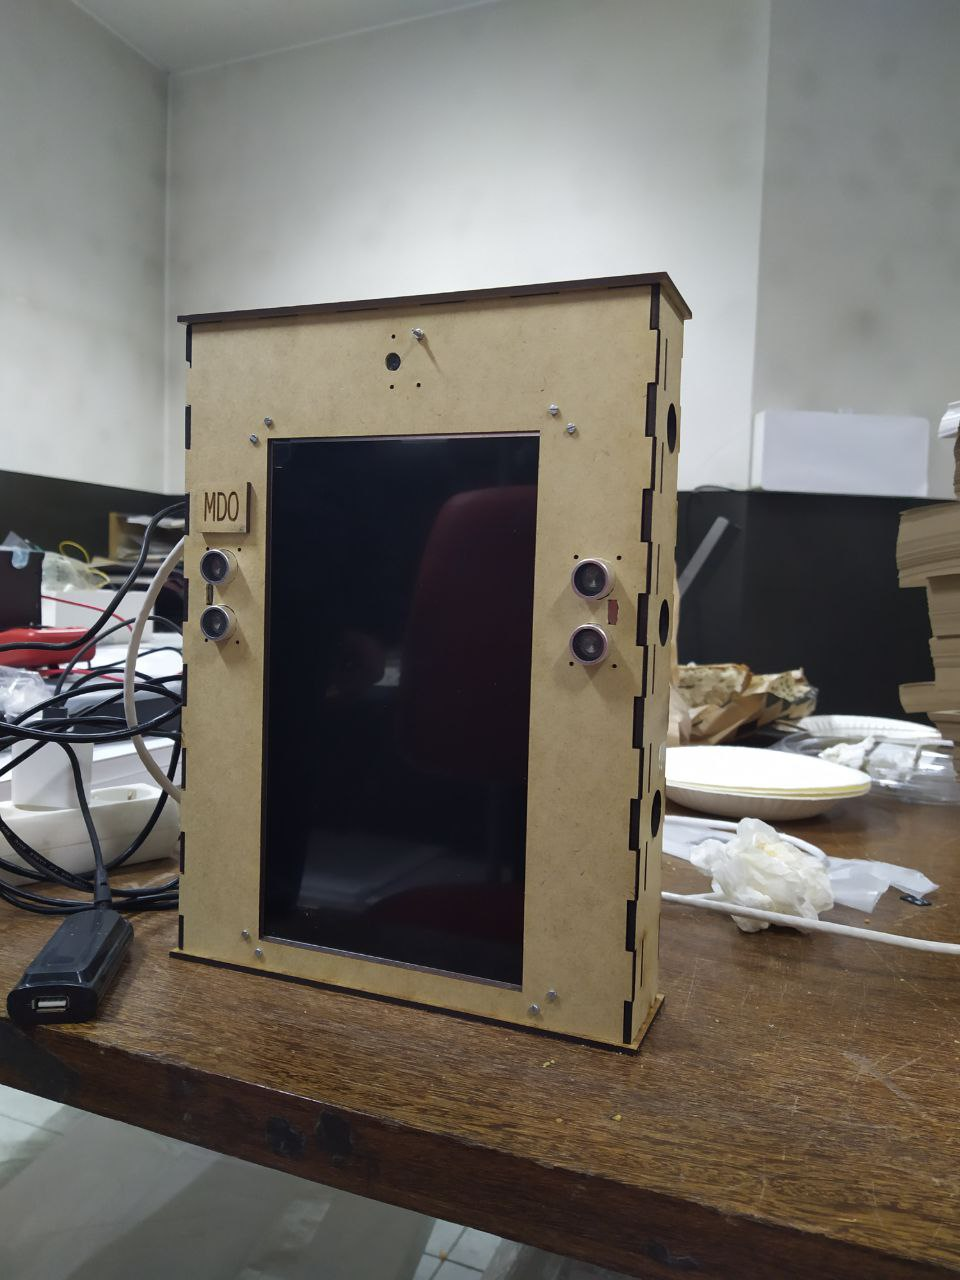
\includegraphics[width=\textwidth]{img/hw-all.jpg}%
  \caption{Login View}%
  \label{fig:hw-all}
\end{subfigure}
%
  \begin{subfigure}{.4\textwidth}
    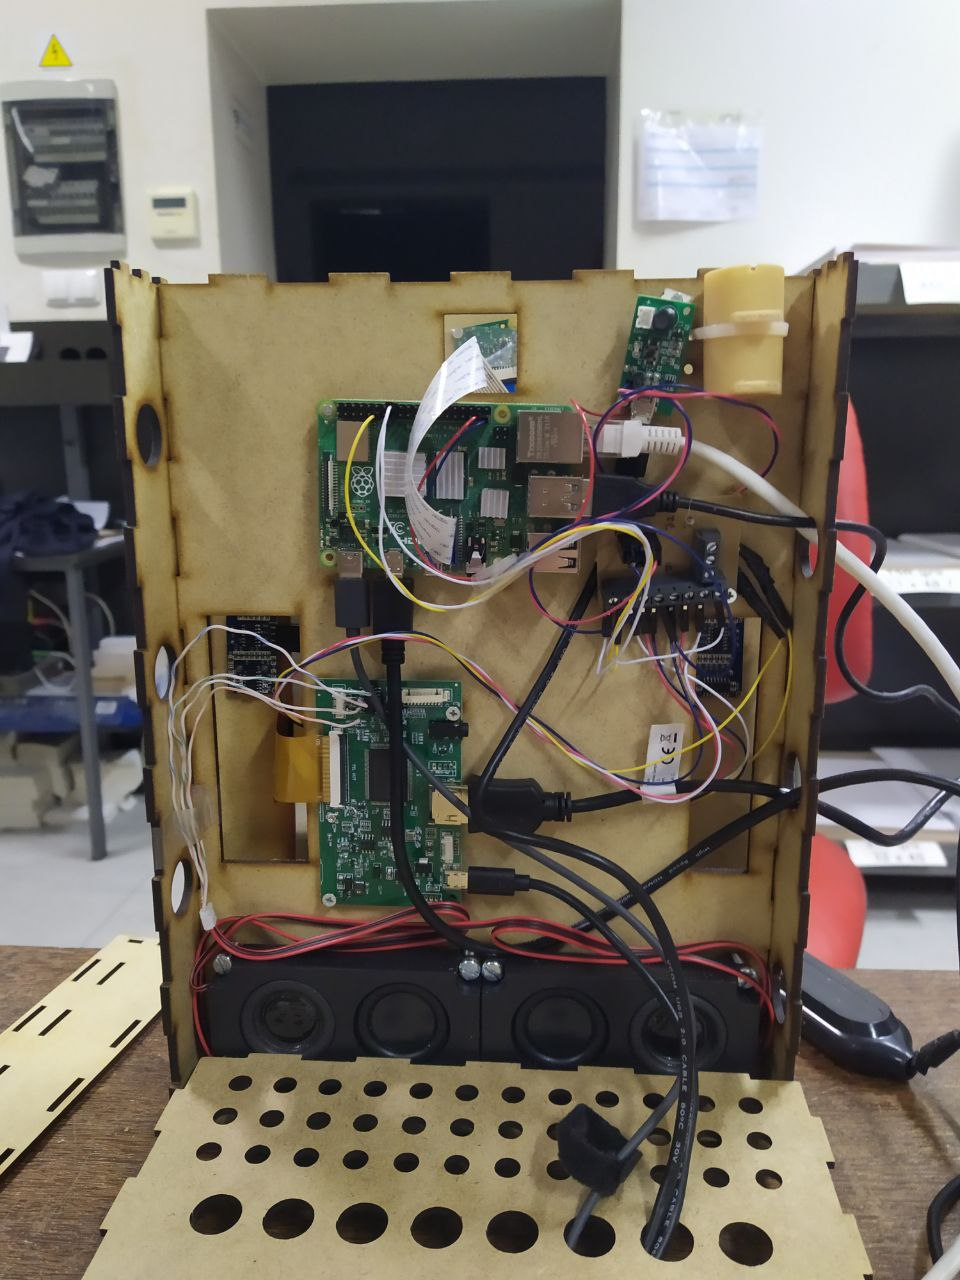
\includegraphics[width=\textwidth]{img/hw-inside.jpg}%
  \caption{Final Hardware Implementation}%
  \label{fig:hw-inside}
  \end{subfigure}
  % 
  \caption{MainWindow views}%
  \label{fig:hw-imp}
\end{figure}
%
\begin{figure}[!htb]
    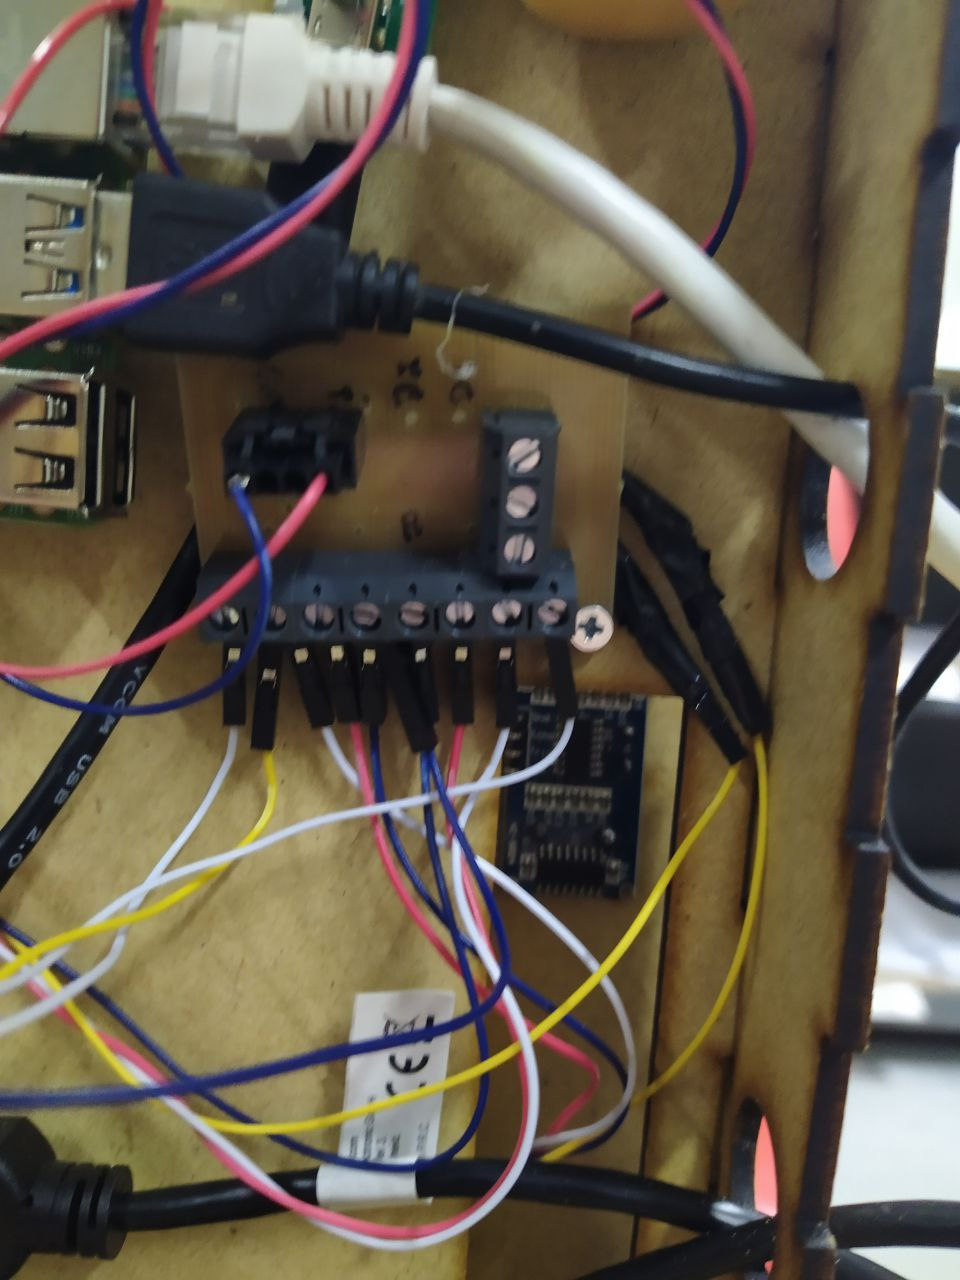
\includegraphics[width=.5\textwidth]{img/pcb.jpg}%
  \caption{Final \gls{pcb}}%
  \label{fig:pcb}
  \end{figure}
%%% Local Variables:
%%% mode: latex
%%% TeX-master: "../../../dissertation"
%%% End:
